\section{Temperature Range of Components}
\label{app:optemp}
\begin{table}[H]
\caption[Operational and Survival Temperature Ranges of various Components]{Operational and Survival Temperature Ranges of various Components \cite{NASAsysreq_Kumar}}
\centering
\begin{tabular}{|l|l|l|}
\hline
\textbf{Component}	&	\textbf{Operational (\si{\degreeCelsius})}	&	\textbf{Survival (\si{\degreeCelsius})}\\\hhline{|=|=|=|}
\textbf{Gears \& Bearings}		&	-25 to 135	&	-50 to 155	\\\hline
\textbf{Motor Windings}			&	-25 to 180	&	-50 to 200	\\\hline
\textbf{Brakes}					&	-25 to 99	&	-50 to 120	\\\hline
\textbf{Cables \& Connectors}	&	-70 to 135	&	-90 to 155	\\\hline
\textbf{Electronics}			&	-20 to 65	&	-50 to 85	\\\hline
\end{tabular}
\end{table}

\subsection*{Data from External Documents}
\begin{figure}[H]
\centering
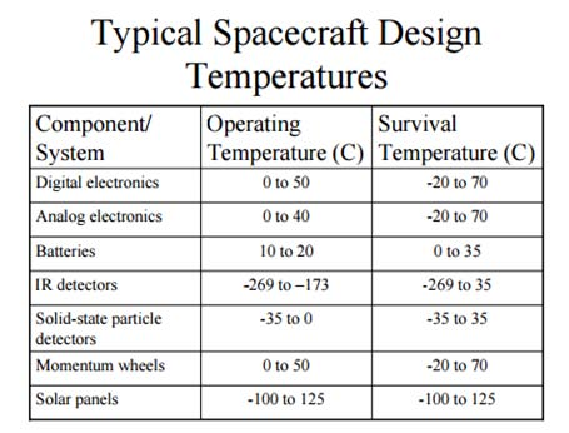
\includegraphics[scale=0.6]{Apppic/designtemp}
\caption[Typical Spacecraft Design Temperatures]{Typical Spacecraft Design Temperatures \cite{spacedesigntemp}}
\end{figure}
\begin{figure}[H]
\centering
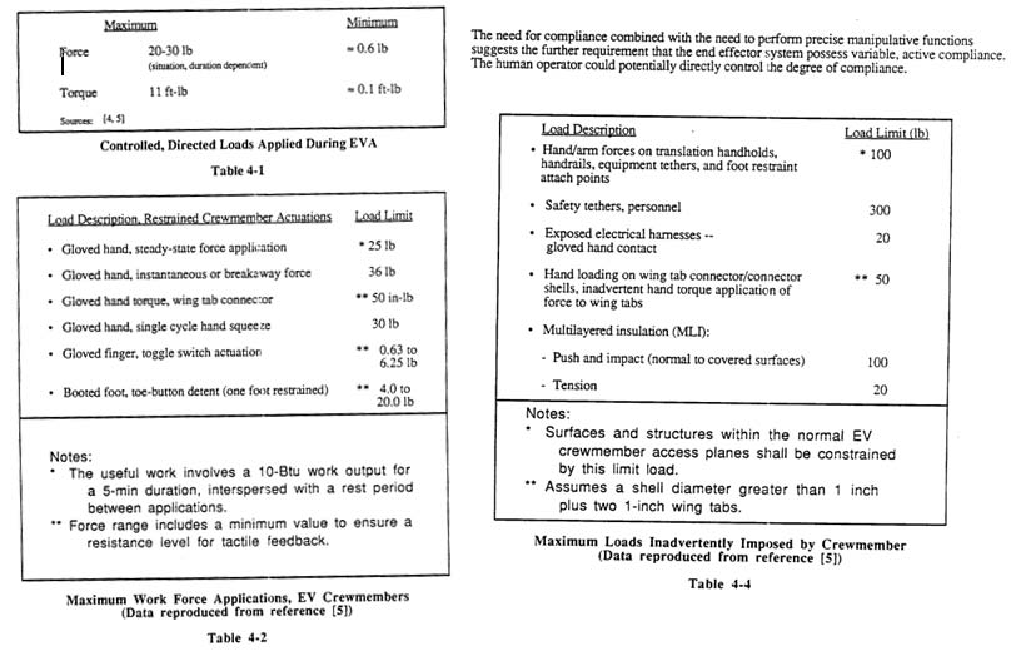
\includegraphics[scale=0.6]{Apppic/eeloads}
\caption[End Effector Load Limits]{End Effector Load Limits \cite{NASAEE_Mishkin}}
\end{figure}
\begin{figure}[H]
\centering
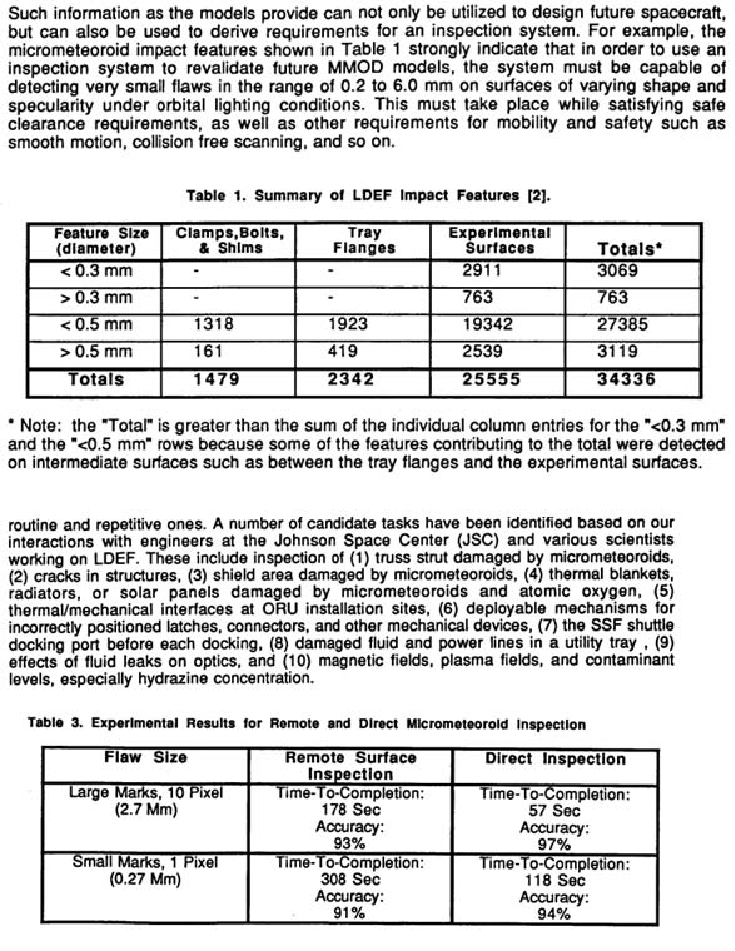
\includegraphics[scale=1]{Apppic/inspect}
\caption[Requirements for Inspection Systems]{Requirements for Inspection Systems \cite{NASAinspect_Hayati}}
\end{figure}